\section{Within-Family Housing Transfers: National Facts}\label{sec:facts}

\paragraph{Fact 1: For every 3.6 market sales, one family-transfer deed is recorded.}
Table~\ref{tab:volumes} and Figure~\ref{fig:volumes} report annual volumes.
Between 0.9 and 1.6 million family-transfer deeds are recorded every year
(same-surname, other-interfamily, and estate/executor), against 3.0 to 5.8 million market
sales: a family:market ratio between 0.25 and 0.34 in every year of the
sample, with a 2007--2023 aggregate of 0.28. The conservative same-surname
series alone runs 0.7 to 1.0 million per year. The channel is not a
recession artifact: the ratio was as high in the 2009 bust (0.29) as in the
2021 boom (0.28). And the count is deliberately strict---it excludes the 12.1
million trust self-transfers, 7.1 million same-person retitles, and 34.0
million other non-market conveyances; adding them, the deed traffic outside
the market rivals the market itself.\footnote{Restricting the denominator to
existing homes (excluding new-construction first sales) raises the aggregate
family:market ratio to 0.30. On a per-property rather than per-deed basis,
the 19.7 million family-transfer deeds cover 16.5 million distinct parcels
(1.19 deeds per parcel).}

\input{tables/T2_volumes.tex}

\begin{figure}[!t]
  \centering
  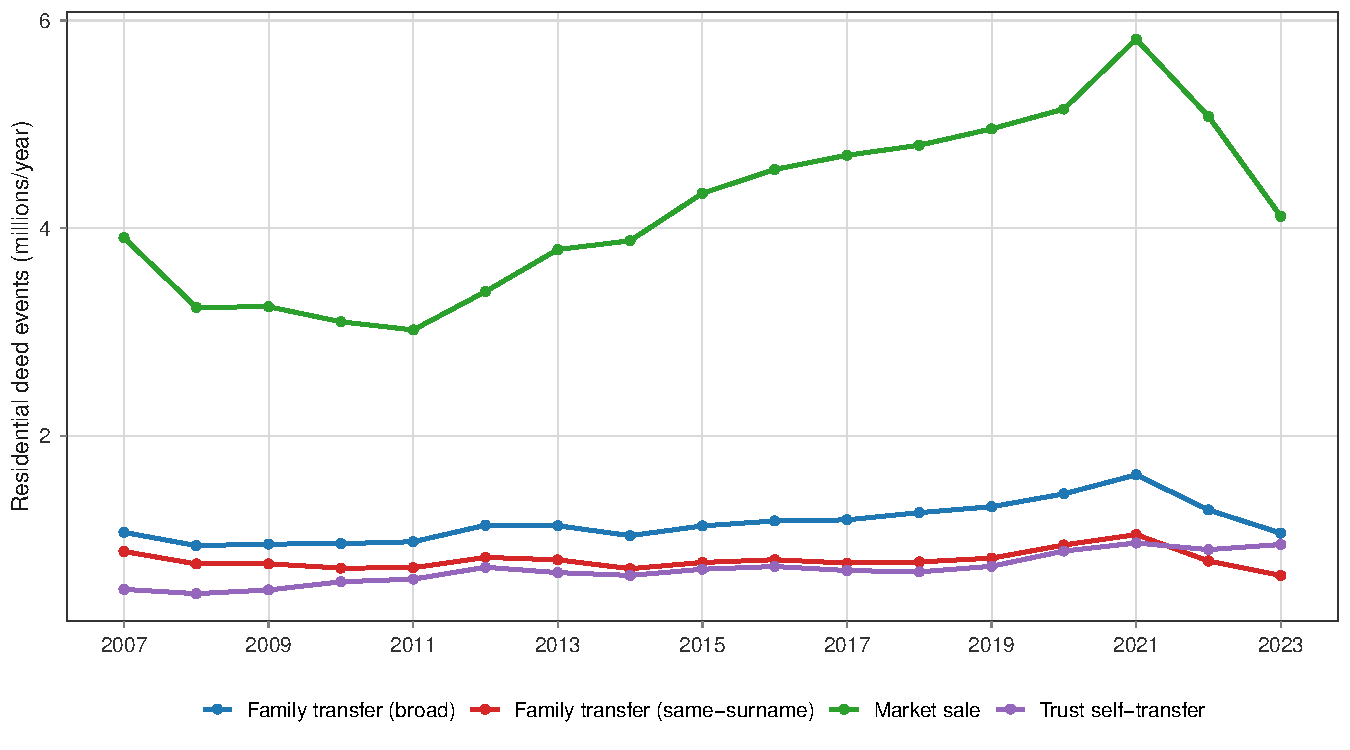
\includegraphics[width=0.92\linewidth]{figures/F1_volumes.pdf}
  \caption{Residential deed events by class, 2007--2023. Family transfer
  (broad) combines same-surname, other-interfamily, and estate/executor
  classes; trust self-transfers are shown separately.}
  \label{fig:volumes}
\end{figure}

\paragraph{Fact 2: Family transfers are concentrated in California.}
Figure~\ref{fig:stateratio} ranks states by the family:market ratio over
2017--2023. California leads the nation at 0.61---one family transfer for
every 1.6 market sales, 2.3 times the pooled national ratio of 0.26---ahead
of Utah and Idaho (0.53). California is exactly where acquisition-value
assessment made the inherited tax basis most valuable, and it also accounts
for 38 percent of all trust self-transfers in the country (2.2 million over
seven years, more than its family transfers), consistent with extensive
estate-planning activity. Cross-state
correlations are not causal evidence---demography, land tenure, and recording
practice all differ---but the cross-section puts the tax-subsidy hypothesis
on the table, and Section~\ref{sec:prop19} tests it within California.

\begin{figure}[!t]
  \centering
  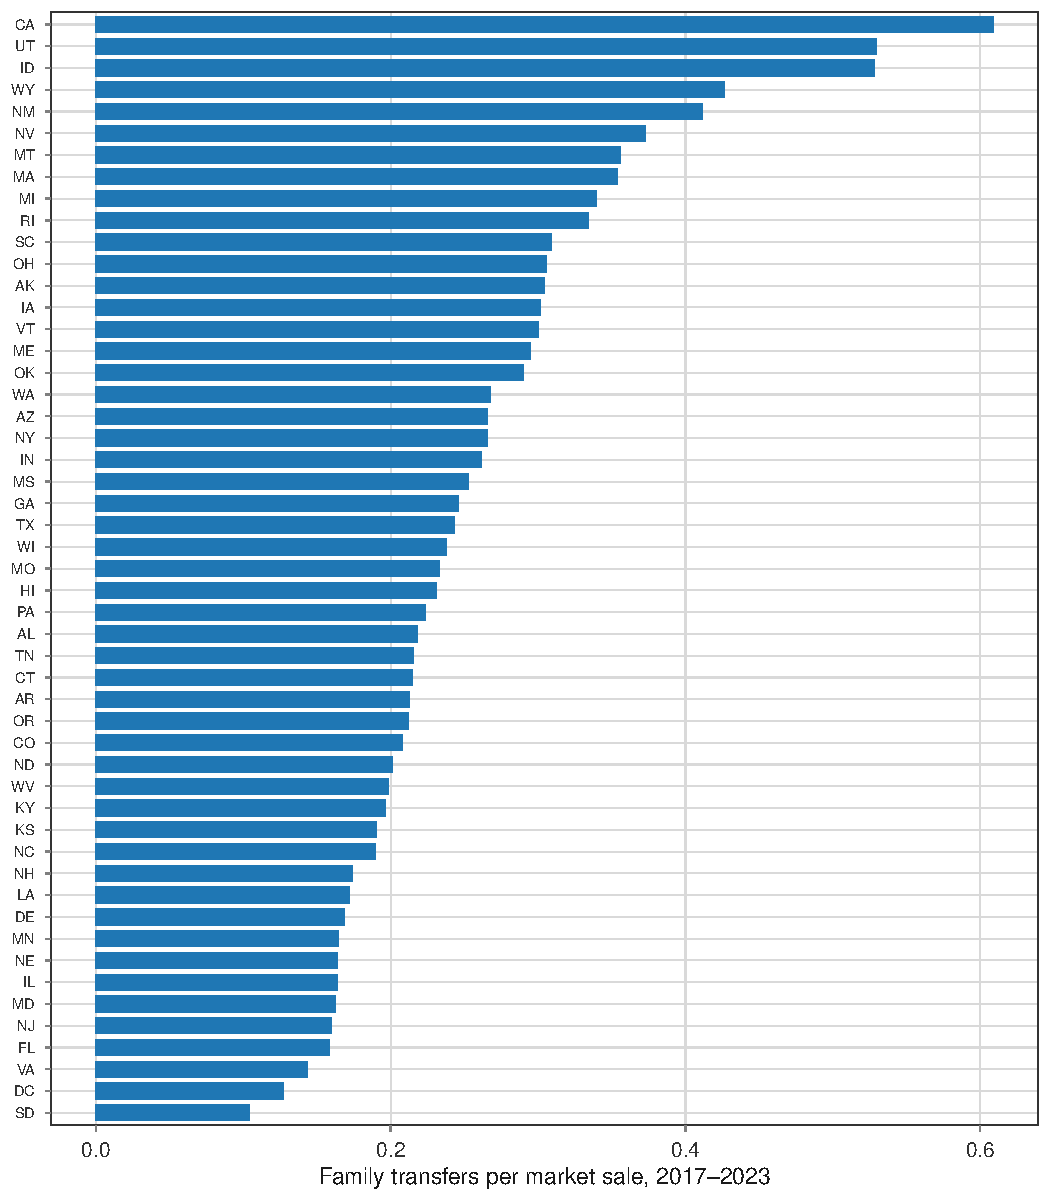
\includegraphics[width=0.78\linewidth]{figures/F2_state_ratio.pdf}
  \caption{Family transfers (broad) per market sale by state, 2017--2023.}
  \label{fig:stateratio}
\end{figure}

\paragraph{Fact 3: Family transfer shares are higher across middle-aged housing vintages.}
Linking deed events to property characteristics (61 percent of 2017--2023
selected family/trust/market events match the available property-characteristics snapshot; Appendix~\ref{app:data}),
the family share of within-class traffic rises with structure age: family
transfers are 20 percent of combined family-plus-market events for houses
of ten to thirty years, 22 percent at thirty to fifty years, and 26 percent
at fifty to seventy-five years, before falling to 24 percent for homes aged 75 or more. The gradient is therefore not monotone over all vintages; the under-ten-year bin also has very few matched events. The family share is higher on parcels with
senior tax exemptions (26 versus 22 percent)---an association measured with a historical snapshot---and declines monotonically across the within-state value
distribution, from 25 percent in the bottom quintile to 21 percent in the
top. The houses that families keep are disproportionately the older, cheaper
stock through which housing filters down to lower-income buyers
\citep{rosenthal2014filtering}.

\paragraph{Property types distinguish different family channels.}
Using recorded land-use codes, family deeds account for 26.6 percent of
combined family-plus-market deeds for duplexes, 23.0 percent for
single-family properties, 15.0 percent for condominiums, and 13.0 percent
for townhouses or rowhouses. On common state-year support, weighting each
type to the single-family distribution leaves the duplex share 2.1
percentage points higher and the condominium and townhouse shares 8.3 and
6.7 points lower, respectively. Appendix~\ref{app:propertytypes} gives the
definitions and denominators. These are static recorded types, not measures
of occupancy or rental use; the apartment sample is selectively covered.
The variation motivates distinguishing inheritance of a residence from
inheritance of housing capital without treating building type as evidence
of either motive.

\paragraph{Fact 4: Three in five family-transferred homes are still unsold a decade later.}
What happens to a house after it enters the family channel? Because the
parcel identifier links successive deeds, every transfer event can be
followed to the property's next arm's-length market sale, if any. We take all
events in the 2008--2018 cohorts---guaranteeing at least 66 months of
follow-up before the June 2024 censoring date---and estimate Kaplan--Meier
survival to first market sale, separately by event class:
8.5 million same-surname family transfers, 3.4 million other family
transfers, 7.1 million trust self-transfers, 4.1 million same-person
retitles, and 42.1 million market purchases as the benchmark.

Table~\ref{tab:hazard} and Figure~\ref{fig:km} show two distinct family
destinies. The first is settlement: among cross-surname family
conveyances---the class containing estate distributions among multiple
heirs---10 percent reach the open market within twelve months and 15 percent
within twenty-four, roughly double the market-purchase benchmark (5 and 9
percent). For a substantial minority, the family deed is the
administrative final step before the house is sold.

The second destiny is the lock. Once a family-transferred home survives the
settlement window, it becomes more immobile than the housing stock at large.
Same-surname transfers start faster than market purchases (\FamilySoldTwo\ versus \MarketSoldTwo
percent sold within two years) but fall behind by year five (\FamilySoldFive\ versus
\MarketSoldFive{} percent) and keep falling behind: by year ten, \FamilySoldTen\ percent of
same-surname family homes have returned to the market against \MarketSoldTen\ percent of
market purchases. Conditional on passing the two-year settlement phase, \FamilyConditionalSold\
percent of family homes sell over the following eight years versus \MarketConditionalSold\
percent of market purchases. The market-purchase benchmark, recall, includes
investors and flippers; family homes are stickier than all of it. Three in
five of the homes that passed between relatives in 2008--2018 had not sold
on the open market a decade later. An internal descriptive check is that
same-person retitles---deeds retaining at least one matched name---track trust self-transfers closely (9.1 versus
8.9 percent sold within two years), consistent with both classes often
recording paperwork rather than a change in the property's use.

This is a descriptive fact, and selection is its content: families keep the
homes they receive. Four caveats discipline its reading. First, the
comparison pools states and cohorts as family transfers concentrate in older
homes and in low-turnover states, so part of the gap is composition. Second, the two clocks
measure different objects: a market purchase starts a fresh tenure, while a
family deed often changes title without changing occupancy---a force that
should, if anything, \emph{raise} the family class's sale hazard, if
family deeds cluster near succession events. Third, some cross-surname
family homes cannot sell for title reasons (heirs' property), a lock of a
different kind \citep{dobbsgaither2023heirs}. Fourth, trust self-transfers
---the trust-keyword class---show survival close to the
same-surname class, a reminder that long-tenure households are exactly the
ones that do estate paperwork. These comparisons do not distinguish attachment, rental use, title constraints, and tax incentives. Proposition~19 identifies a response of deeds to a policy change; additional assumptions are needed to connect that response to allocation.

\input{tables/T3_hazard.tex}

\begin{figure}[!t]
  \centering
  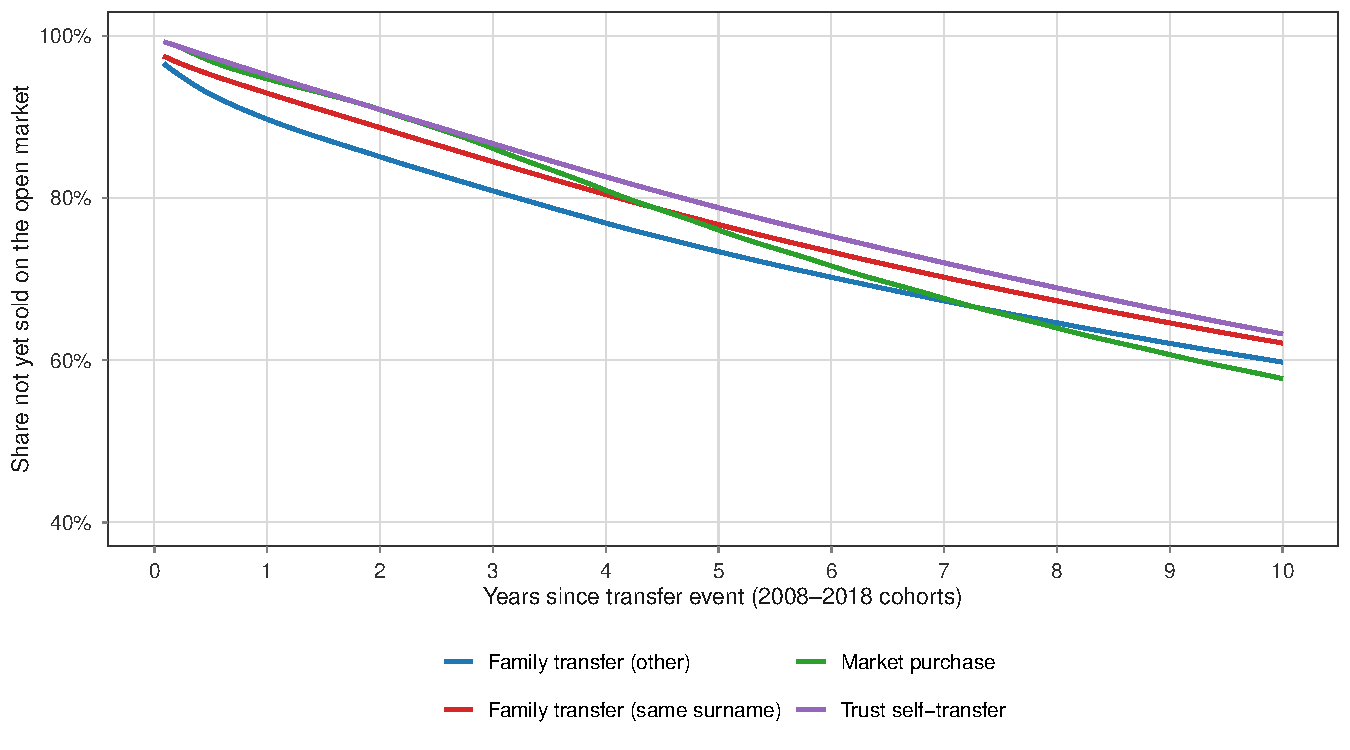
\includegraphics[width=0.92\linewidth]{figures/F3_km_curves.pdf}
  \caption{Kaplan--Meier survival to first open-market sale, 2008--2018
  event cohorts, censored June 2024. The estate/executor class
  (n=665) is omitted.}
  \label{fig:km}
\end{figure}
